The SWCNTs become unstable when exposed to air; for this reason, a lipophilic membrane was prepared and dropcasted on the channel.
The membrane is composed of 5\% (\SI{5.01}{\mg}) tetradodecylammonium tetrakis(4-chlorophenyl) borate, 32.3\% (\SI{32.36}{\mg}) poly(vinyl chloride) (PVC), and 62.7\% (\SI{62.83}{\mg}, \ie{} \SI{0.137}{\ml}) dioctyl sebacate (Merck) dissolved in \SI{1}{\ml} of tetrahydrofuran (THF). The mixture was sonicated \SI{5}{\min}, then vortexed until most powder was dissolved (approximately \SI{5}{\min}) and finally put in the ultrasound sonicator for additional \SI{30}{\min} to ensure proper mixing. Once prepared, the membrane solution was stored up to \SI{6}{months} at \SI{4}{\degreeCelsius} in a vial sealed with parafilm to prevent THF evaporation. 
Before use, the membrane needed to be sonicated for \SI{1}{\min} to make it homogenous again, then it needed to be placed in ice to cool; this prevented rapid THF evaporation allowing more working time, thus ensuring a more even deposition. The dropcasting itself needed optimization to find complete coverage of the CNT channel. Initially, a single-step deposition of \SI{10}{\ul} was attempted, but it was found to lead to an inconsistent coverage (results are discussed in Section \ref{sec:membrane_encapsulation}, Figure \ref{fig:membrane10ul}). For the complete coverage of the channel, it was found that a two-step process was more convenient: first, \SI{8}{\ul} of membrane solution were dropcasted over the channel and left to dry for \SI{30}{\min}; then, an additional \SI{7}{\ul} were deposited on top of the first layer. This approach allowed for a thicker and more protective layer while still allowing current to flow in the channel.

The membrane was later characterized using optical microscopy and profilometry to assess its uniformity and thickness (see Figure \ref{fig:membrane}). These measurements were performed with a KLA Tencor P-6 Surface Profilometer equipped with a \SI{2.0}{\um} diamond stylus. The samples were fixed onto the stage using a vacuum system, and measurements were conducted with a scan speed of \SI{50}{\um\per\second}, a sampling rate of \SI{50}{\hertz}, and an applied stylus force of \SI{2.0}{\mg}.

\begin{figure}
    \centering
    \subfloat[Optical microscopy]{
        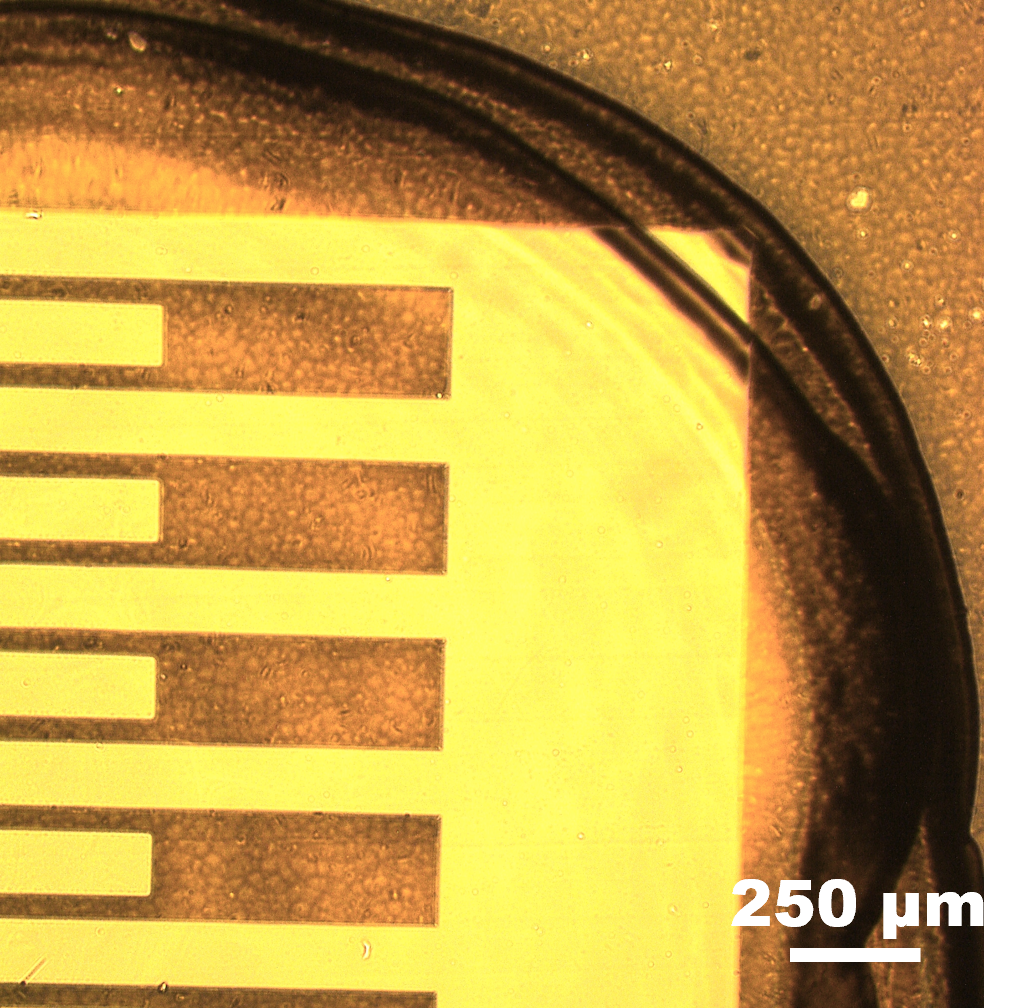
\includegraphics[width=0.3\textwidth]{figures/chapter2/membrane/Fig_channelMembrane.png}
    } \quad
    \subfloat[Profilometry]{
        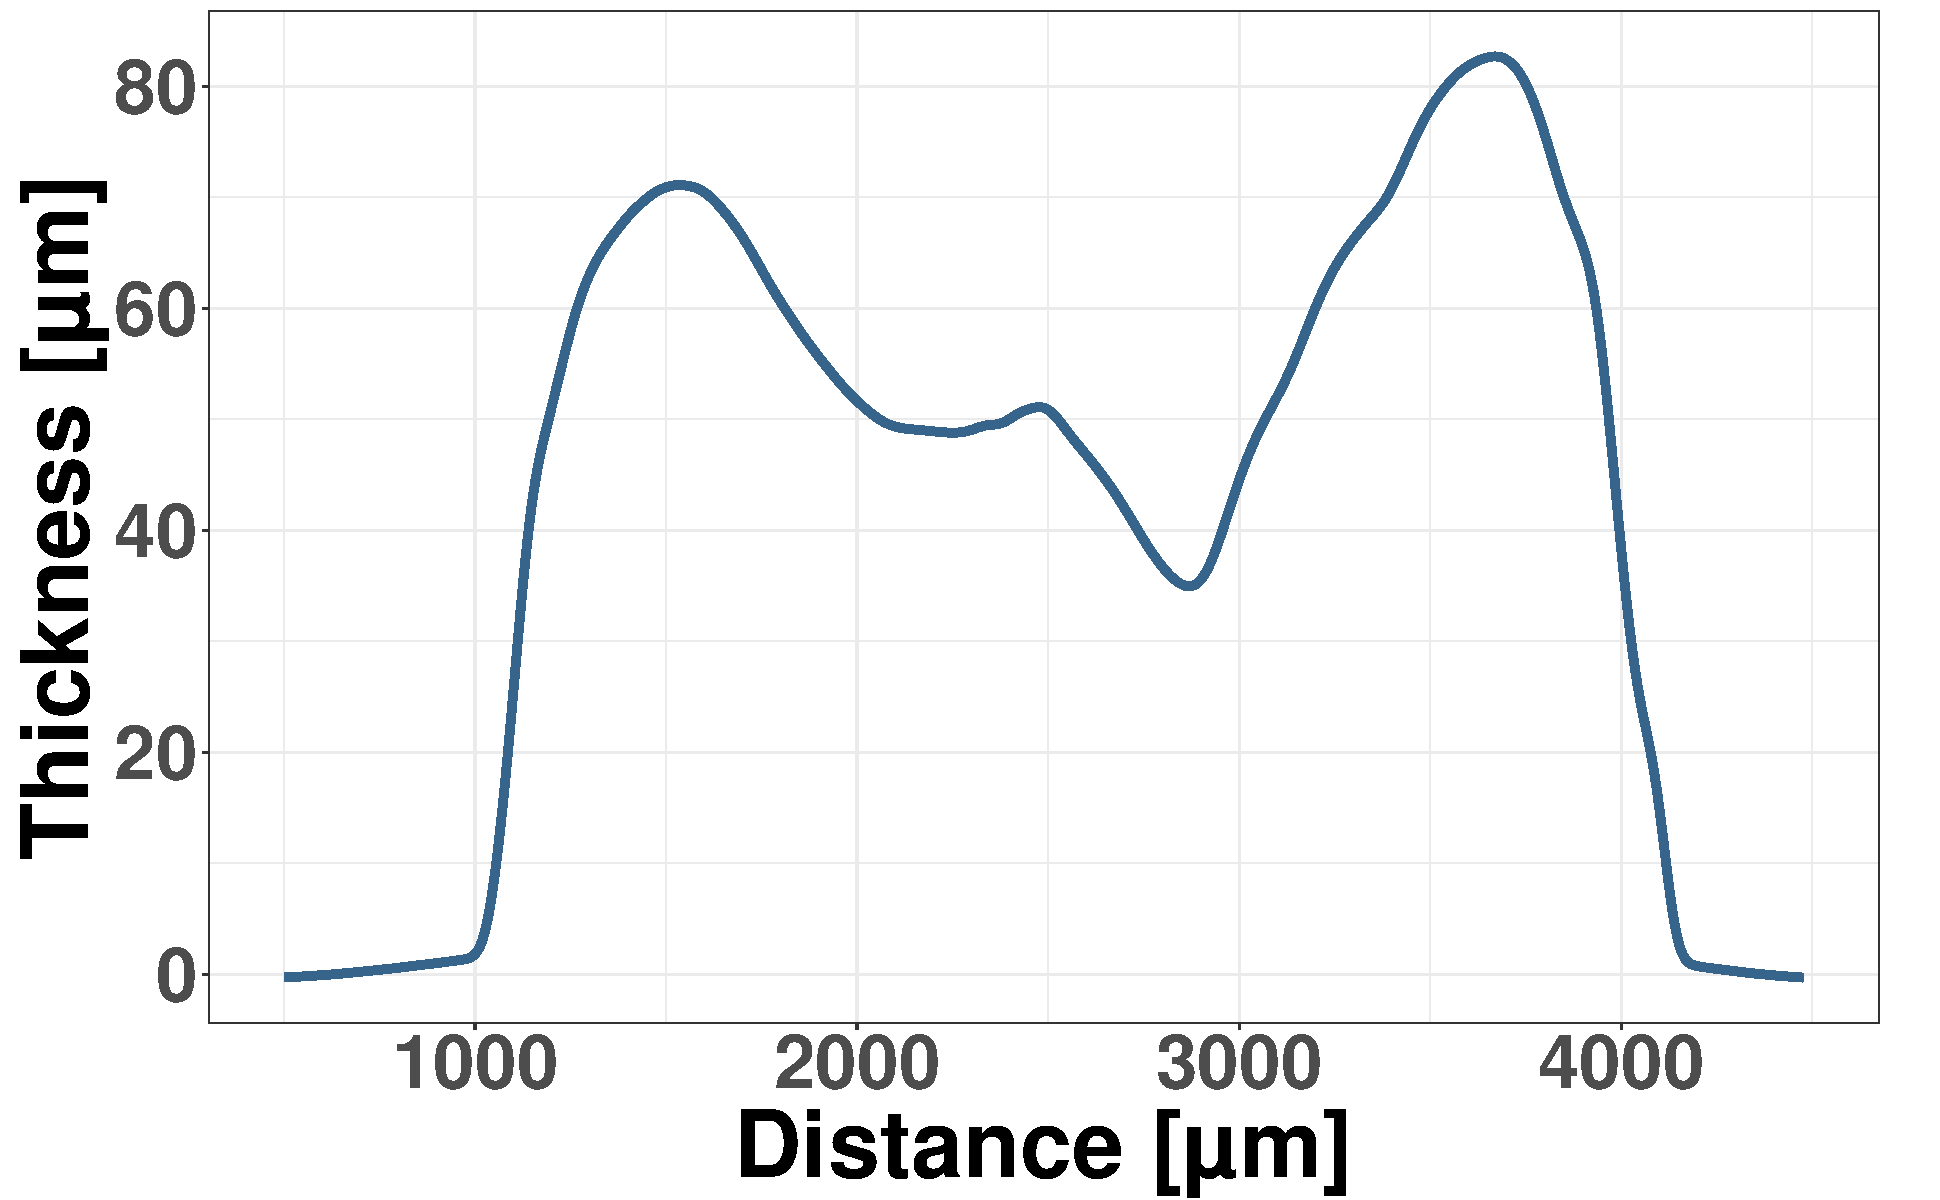
\includegraphics[width=0.4\textwidth]{figures/chapter2/membrane/Fig_channelMembraneProfil.pdf}
    }
    \caption{Morphological characterization of the channel membrane. 
    (a) At the optical microscope, the membrane appears transparent, and the underlying IDEs are still clearly visible; it is still possible to see the borders, where the double line is a sign of the two-step deposition. 
    (b) The analysis of the membrane profile shows an average thickness of \SI{46.33 \pm 19.74}{\um}, while also indicating the presence of a slight coffee ring effect; indeed, the membrane is thicker at the borders, while being slightly thinner at the center.}
    \label{fig:membrane}
\end{figure}
